\documentclass[12pt]{article}

% ----------------------------------------------------------
% Packages
% ----------------------------------------------------------
\usepackage{amsmath, amssymb, amsfonts}
\usepackage{graphicx}
\usepackage{booktabs}
\usepackage{geometry}
\usepackage{hyperref}
\usepackage{setspace}
\usepackage{float}
\usepackage{caption}
\usepackage{subcaption}
\usepackage{array}
\usepackage{longtable}
\usepackage{adjustbox}
\usepackage{microtype}
\usepackage{enumitem}
\usepackage{tabularx}
\usepackage[numbers, square]{natbib}

% GRAPHING PACKAGES
\usepackage{tikz}
\usepackage{pgfplots}
\pgfplotsset{compat=1.18}
\usetikzlibrary{patterns}

\geometry{margin=1in}
\onehalfspacing

% flexible column type for descriptions
\newcolumntype{Y}{>{\raggedright\arraybackslash}X}

% ----------------------------------------------------------
% Title
% ----------------------------------------------------------
\title{\textbf {An Exhaustive Analysis on Decline of the Labor Share in India (Sinha 2023)}}
\date{}
% ----------------------------------------------------------
\begin{document}
\maketitle
\vspace{-2cm}
\begin{abstract}
This document provides an exhaustive analysis of the decline of the labor share in India, synthesizing empirical evidence, decompositional accounting, econometric estimation of markups, and a calibrated three-sector general equilibrium model. The report evaluates competing hypotheses — Investment-Specific Technical Change (ISTC) driven by a fall in the Relative Price of Investment and the Market Power / rising-markups hypothesis — and performs a quantitative horse race between calibrated counterfactuals. The analysis highlights the role of India's unusual structural transformation (a services leap) and the interplay of substitution and income effects.
\end{abstract}

\tableofcontents
\newpage

% ----------------------------------------------------------
\section{Introduction}
The functional distribution of income—the division of national economic output between the factors of production, labor and capital—has transitioned from a parameter of assumed stability to a central variable of macroeconomic inquiry. For the better part of the twentieth century, the constancy of the labor share of income was enshrined as one of Nicholas Kaldor’s stylized facts of economic growth, providing a convenient empirical anchor for Cobb–Douglas production functions and standard growth models. However, the empirical consensus has fractured over the last four decades. A robust body of literature now documents a secular and pervasive decline in the labor share across both advanced and developing economies, challenging the neutrality of technological progress and raising profound questions regarding inequality, market structure, and the future of work.

Within this shifting global landscape, the Indian economy presents a case study of singular complexity and theoretical significance. As elucidated in the focal research by Sinha (2023), India has witnessed a precipitous contraction in its aggregate labor share of income—a decline of approximately seven percentage points over a thirty-year horizon from the early 1980s to the late 2000s. This decline is not merely a statistical artifact; it represents a fundamental alteration in the rewards to production during a period of rapid economic liberalization and growth.

The Indian experience is analytically distinct due to the idiosyncrasy of its development trajectory. Standard structural transformation models posit a linear progression where labor migrates from low-productivity agriculture to high-productivity manufacturing, and eventually to services—a path exemplified by the East Asian Tigers. India, however, has defied this canonical sequence, exhibiting a leapfrog pattern where the economy transitioned directly from an agrarian base to a service-led growth model, bypassing the mass industrialization phase typically associated with labor absorption.

This report provides an exhaustive analysis of the causes, mechanisms, and implications of India's declining labor share. Synthesizing the findings of Sinha (2023) with a broader array of development literature and econometric evidence, this document dissects the interplay between two dominant global hypotheses: the technological explanation rooted in the decline of the Relative Price of Investment (RPI), and the market-structure explanation rooted in rising firm markups.
\newpage
\subsection{Research Objective and Scope}
The primary objective of this report is to rigorously evaluate the causal architecture of India's factor share dynamics. The inquiry is structured around three core investigative pillars:
\begin{enumerate}[leftmargin=*,itemsep=4pt]
\item \textbf{Decomposition and Anatomy:} Dissect the aggregate decline into its constituent parts—specifically distinguishing between the impact of falling labor shares within industries (the LS Effect) and the impact of the reallocation of economic activity between industries (the VA Effect and Covariance Term).
\item \textbf{Causal Mechanisms (The Horse Race):} Adjudicate between the competing hypotheses of Investment-Specific Technical Change (ISTC), which posits that cheaper capital goods drive capital–labor substitution, and the Market Power hypothesis, which attributes the decline to rising profit wedges.
\item \textbf{Structural Interaction:} Elucidate how India’s unique pattern of structural change—specifically the expansion of the services sector—interacts endogenously with these macroeconomic forces.
\end{enumerate}

The analysis draws upon a rich dataset comprising the India KLEMS database, the Annual Survey of Industries (ASI), and supplementary research on Indian labor markets and trade policy. By reconstructing the theoretical architecture of Sinha's three-sector General Equilibrium (GE) model and critically evaluating its calibration and counterfactuals, this report argues that the decline in the relative price of investment, interacting with non-homothetic preferences, offers the most parsimonious and robust explanation for the observed phenomena. Furthermore, the report extends the analysis to address critical gaps in the primary literature, specifically the role of the unorganized (informal) sector and the nuances of labor regulation in India.

\newpage
% ----------------------------------------------------------
\section{The Empirical Landscape: Data, Trends, and Stylized Facts}

A rigorous investigation into factor shares in a developing economy requires a nuanced understanding of the underlying data infrastructure. The measurement of labor share is fraught with definitional challenges, particularly in economies with large self-employed populations where mixed income blurs the distinction between wage and profit.

\subsection{The Data Architecture: KLEMS and ASI}

\subsubsection{The India KLEMS Database}
Constructed by the Reserve Bank of India (RBI), the KLEMS database provides the macroeconomic aggregate view. It offers harmonized time-series data on Gross Value Added (GVA), labor input, capital input, and factor income shares for 27 distinct industries. The strength of the KLEMS data lies in its methodological consistency, allowing for the construction of long-run time series (1980–2011) that account for the changing composition of the economy. Crucially, the KLEMS methodology adjusts for the mixed income of the self-employed, typically by imputing wages based on the earnings of similarly skilled hired workers—a necessary correction in the Indian context where self-employment is pervasive.

\subsubsection{The Annual Survey of Industries (ASI)}
While KLEMS provides the sectoral view, the ASI provides the micro-foundations. The ASI is the primary source of industrial statistics in India, covering the organized manufacturing sector. It utilizes a dual-sampling strategy: a Census sector comprising larger units (typically those with more than 100 or 200 workers, depending on the year) which are surveyed completely, and a Sample sector of smaller units surveyed probabilistically. Sinha (2023) utilizes the ASI specifically to construct a firm-level panel for the estimation of production functions and markups. The creation of a longitudinal panel from ASI data is a non-trivial econometric task, as the survey does not historically maintain unique firm identifiers across years. The analysis employs a matching algorithm based on time-invariant characteristics—such as the year of initial production, location codes, and industry classification—to link observations, achieving a match rate of approximately 36\%.

\subsection{Stylized Fact 1: The Sectoral Heterogeneity of the Decline}
The aggregate labor share in India fell from approximately 55.47\% in 1980 to 48.5\% in 2011. This 6.9 percentage point decline is the central estimand of the research. However, this aggregate figure masks profound heterogeneity at the sectoral level.

% ----------------------------------------------------------
% GRAPH 1: SECTORAL LABOR SHARE COMPARISON
% ----------------------------------------------------------
\begin{figure}[H]
\centering
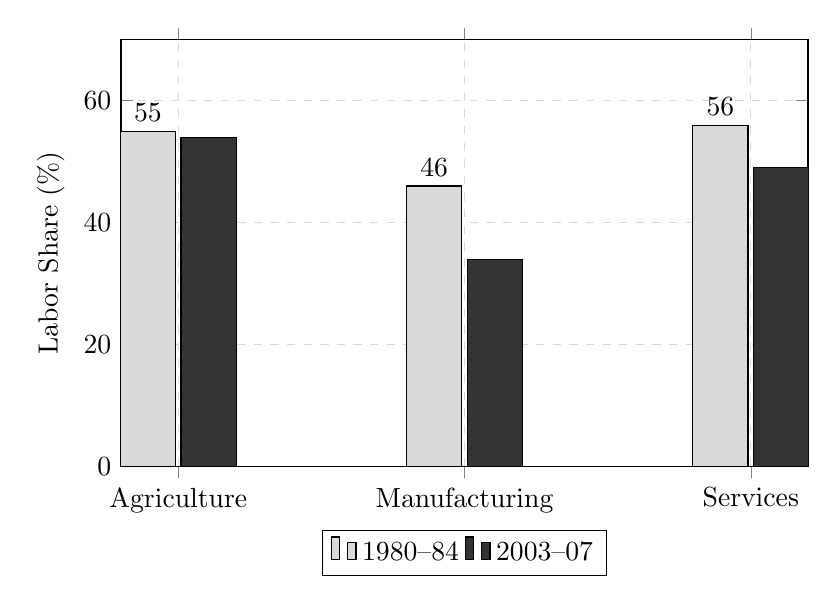
\begin{tikzpicture}
    \begin{axis}[
        ybar,
        bar width=20pt,
        width=0.85\textwidth,
        height=7cm,
        symbolic x coords={Agriculture, Manufacturing, Services},
        xtick=data,
        ylabel={Labor Share (\%)},
        ymin=0, ymax=70,
        nodes near coords,
        legend style={at={(0.5,-0.15)}, anchor=north, legend columns=-1},
        grid=major,
        major grid style={dashed, gray!30}
    ]
    % 1980 Data
    \addplot[fill=gray!30, draw=black] coordinates {(Agriculture,55) (Manufacturing,46) (Services,56)};
    % 2007 Data
    \addplot[fill=black!80, draw=black, text=white] coordinates {(Agriculture,54) (Manufacturing,34) (Services,49)};
    
    \legend{1980--84, 2003--07}
    \end{axis}
\end{tikzpicture}
\caption{Evolution of Labor Share by Sector. Note the steep decline in Manufacturing.}
\label{fig:sector_ls}
\end{figure}
% ----------------------------------------------------------

\begin{table}[H]
\centering
\caption{Sectoral Labor Share Dynamics (1980--2007)}
\begin{tabular}{lccc}
\toprule
Sector & Labor Share (1980--84) & Labor Share (2003--07) & Change ($\Delta$) \\
\midrule
Agriculture & 55\% & 54\% & $-1$ pp \\
Manufacturing & 46\% & 34\% & $-12$ pp \\
Services & 56\% & 49\% & $-7$ pp \\
\bottomrule
\end{tabular}
\end{table}

The data reveals a stark bifurcation. The agricultural sector, which remains the largest employer in terms of headcount, experienced virtually no change in its functional income distribution. In contrast, the modern sectors—Manufacturing and Services—witnessed significant declines. The Manufacturing sector’s decline is particularly acute, falling by 12 percentage points. This suggests that the drivers of the labor share decline are intrinsic to the capitalist, formal segments of the economy where capital–labor substitution is technologically feasible.

\subsection{Stylized Fact 2: The Anomaly of Structural Transformation}
The second defining feature of the Indian economy during this period is its unique structural transformation. Standard development theory anticipates a transition where the manufacturing sector's share of GDP rises significantly (industrialization) before eventually yielding to services. India deviated from this path.

% ----------------------------------------------------------
% GRAPH 2: STRUCTURAL TRANSFORMATION
% ----------------------------------------------------------
\begin{figure}[H]
\centering
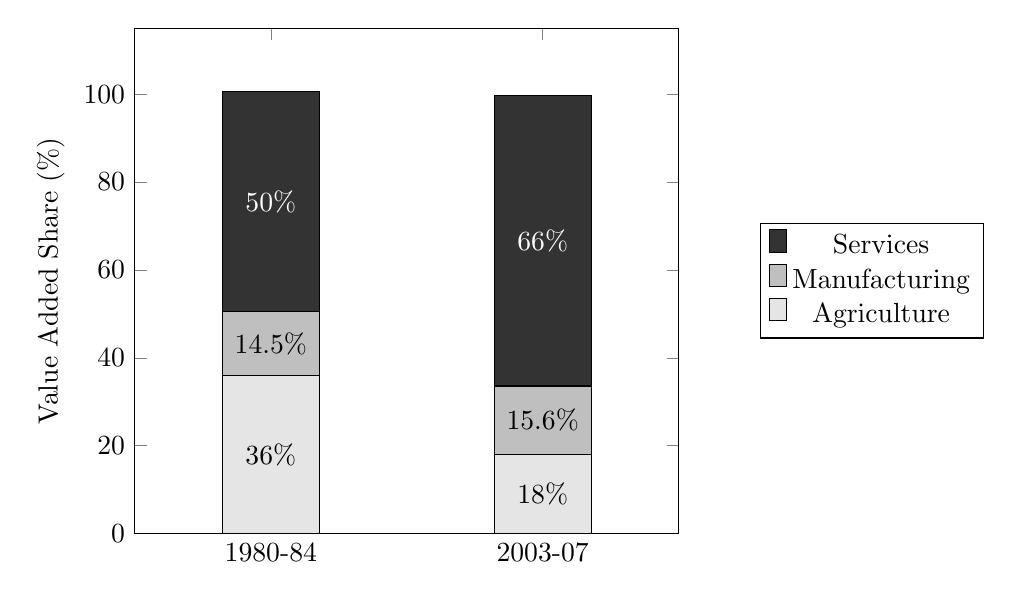
\begin{tikzpicture}
    \begin{axis}[
        ybar stacked,
        bar width=35pt,
        width=0.7\textwidth,
        height=8cm,
        symbolic x coords={1980-84, 2003-07},
        xtick=data,
        enlarge x limits=0.5,
        ylabel={Value Added Share (\%)},
        ymin=0, ymax=115,
        legend style={at={(1.15,0.5)}, anchor=west},
        reverse legend,
        nodes near coords={%
            \pgfmathprintnumber[fixed, precision=1]{\pgfplotspointmeta}\%
        },
        nodes near coords align={center},
    ]
    % Stacked Plots
    \addplot[fill=black!10, draw=black] coordinates {(1980-84,36) (2003-07,18)}; % Ag
    \addplot[fill=gray!50, draw=black] coordinates {(1980-84,14.5) (2003-07,15.6)}; % Mfg
    \addplot[fill=black!80, draw=black, text=white] coordinates {(1980-84,50) (2003-07,66)}; % Svc
    
    \legend{Agriculture, Manufacturing, Services}
    \end{axis}
\end{tikzpicture}
\caption{The Services Leap: Structural Transformation of the Indian Economy.}
\label{fig:structure}
\end{figure}
% ----------------------------------------------------------

\begin{table}[H]
\centering
\caption{Structural Transformation - Value Added Shares (1980--2007)}
\begin{tabular}{lccc}
\toprule
Sector & Value Added Share (1980--84) & Value Added Share (2003--07) & Change ($\Delta$) \\
\midrule
Agriculture & 36\% & 18\% & $-18$ pp \\
Manufacturing & 14.5\% & 15.6\% & $+1.1$ pp \\
Services & 50\% & 66\% & $+16$ pp \\
\bottomrule
\end{tabular}
\end{table}

As illustrated above, the Manufacturing sector's share of value added remained virtually stagnant, hovering around 15\%. The vacuum created by the contraction of Agriculture (from 36\% to 18\%) was filled almost entirely by the Services sector, which expanded from 50\% to 66\% of the economy. This Services Leap is critical because it alters the weighted average of the aggregate labor share. If the economy shifts resources into a sector with a lower (or falling) labor share, the aggregate labor share will decline even if within-sector shares remain constant.

\subsection{Stylized Fact 3: The Positive Covariance Puzzle}
The most sophisticated empirical insight from the preliminary data analysis is the identification of a strong positive covariance between sector size growth and labor share decline. It is not merely that the labor share fell, or that the service sector grew; it is that the sectors that were growing the fastest (Services) were precisely the sectors experiencing a decline in their labor share.

This relationship demands a unified theoretical explanation. A stochastic model where labor shares and sectoral shares evolve independently would fail to capture this systematic correlation. The challenge for any theoretical model is to identify a mechanism that simultaneously incentivizes firms to reduce their wage bill share and incentivizes households to shift their consumption basket toward the output of those very firms.

\newpage
% ----------------------------------------------------------
\section{Global Debate on Factor Shares}

To interpret the Indian data, we must situate it within the broader theoretical debate regarding the global decline of the labor share. Two primary hypotheses have emerged in the macro-labor literature: the technological explanation centered on relative prices, and the institutional explanation centered on market power.

\subsection{The Investment-Specific Technical Change (ISTC) Hypothesis}
The leading technological explanation, advanced prominently by Karabarbounis and Neiman (2013) \citep{Karabarbounis2013}, posits that the decline in the labor share is driven by the decline in the Relative Price of Investment (RPI) goods. This hypothesis rests on the concept of Investment-Specific Technical Change (ISTC)—advancements in the production of capital goods (computers, machinery, software) that make them cheaper relative to consumption goods.

\paragraph{The Mechanism of Substitution}
The transmission mechanism relies on the elasticity of substitution between capital and labor ($\sigma$). In a standard Constant Elasticity of Substitution (CES) production framework, the response of factor shares to a change in factor prices is determined by whether capital and labor are gross substitutes ($\sigma > 1$) or gross complements ($\sigma < 1$).
\begin{itemize}[leftmargin=*,itemsep=4pt]
\item \textbf{Price Effect:} A decline in the RPI lowers the user cost of capital ($R$).
\item \textbf{Quantity Effect:} Firms respond by accumulating more capital ($K$).
\item \textbf{Net Effect on Shares:}
\begin{itemize}
\item If $\sigma > 1$, the increase in capital usage ($K$) outweighs the decline in its price ($R$). The total payment to capital ($RK$) rises relative to total output ($PY$), causing the capital share to rise and the labor share to fall.
\item If $\sigma < 1$, the accumulation of capital is insufficient to offset the price decline. The capital share falls, and the labor share rises.
\end{itemize}
\end{itemize}

\paragraph{Relevance to India}
This hypothesis is particularly pertinent to India due to the shock of the 1991 liberalization. Prior to 1991, India operated under a regime of capital import substitution, characterized by high tariffs and quantitative restrictions on the import of machinery. As documented by Johri and Rahman (2022) \citep{JohriRahman2022}, the relative price of investment in India rose by 44\% from 1981 to 1991 due to these scarcity-inducing policies. The 1991 reforms, which slashed tariffs and dismantled licensing regimes, reversed this trend, causing the RPI to fall by approximately 26\% to 31\% between 1991 and 2006. Sinha (2023) estimates an even sharper decline of nearly 50\% when extending the data to 2011 using Penn World Tables. This dramatic, policy-induced variation in relative prices provides a potent natural experiment to test the substitution hypothesis.

\subsection{The Market Power and Markup Hypothesis}
The competing hypothesis, championed by De Loecker, Eeckhout, and Unger (2020) \citep{DeLoecker2020}, argues that the decline in the labor share is not a technological phenomenon but a market structure phenomenon. This view posits that the rise of superstar firms, network effects, and weak antitrust enforcement has led to a secular increase in aggregate markups.

\paragraph{The Mechanism of the Profit Wedge}
The labor share ($LS$) can be expressed as the ratio of the output elasticity of labor ($\theta_L$) to the markup ($\mu$):
\[
LS = \frac{WL}{PY} = \frac{\theta_L}{\mu}
\]
Even if technology ($\theta_L$) remains constant, an increase in the markup $\mu$ (Price / Marginal Cost) will mechanically depress the labor share. The revenue generated by the markup wedge accrues to firm owners as pure economic profit (rents), squeezing the slice of the pie available for both labor and capital remuneration.

\paragraph{Relevance to India}
The applicability of this hypothesis to India is a subject of debate. The Indian economy of the 1980s was characterized by the License Raj, a system that severely restricted entry and competition, fostering highly concentrated, monopolistic markets. Consequently, markups in pre-liberalization India were likely already high. The liberalization of 1991, by opening the economy to foreign competition and domestic entry, would theoretically be expected to reduce markups, which would—all else equal—increase the labor share. Investigating this hypothesis requires rigorous econometric estimation of markups to determine if the Indian trajectory mirrors the rising-markup trend observed in the US and Europe.

\newpage
% ----------------------------------------------------------
\section{Decomposition Analysis: Anatomy of the Decline}

Before deploying a theoretical model, it is essential to perform a rigorous accounting decomposition of the aggregate labor share decline. Sinha (2023) employs a shift–share analysis to partition the total change in the labor share ($\Delta LS$) into three additive components: the Within-Industry Effect, the Between-Industry (Structural Change) Effect, and the Interaction (Covariance) Effect.

\subsection{The Decomposition Methodology}
Let $LS_t$ denote the aggregate labor share at time $t$, $ls_{i,t}$ the labor share in sector $i$, and $v_{i,t}$ the value-added share (weight) of sector $i$.

\[
LS_t = \sum_{i} v_{i,t} \, ls_{i,t}
\]

The change in the aggregate labor share over a period is decomposed as follows:

\[
\Delta LS = \underbrace{\sum_{i} v_{i,0} \Delta ls_{i}}_{\text{LS Effect}} +
\underbrace{\sum_{i} ls_{i,0} \Delta v_{i}}_{\text{VA Effect}} + \underbrace{\sum_{i} \Delta v_{i} \Delta ls_{i}}_{\text{Covariance Term}}
\]

\paragraph{Interpretation}
\begin{itemize}[leftmargin=*,itemsep=4pt]
\item \textbf{LS Effect (Within-Industry):} Captures the contribution of falling labor shares inside individual firms and industries, holding the economy’s structure constant at the base year. This component proxies for forces like capital–labor substitution or rising firm-level markups.
\item \textbf{VA Effect (Structural):} Captures the contribution of the reallocation of economic activity from high-labor-share sectors to low-labor-share sectors, holding within-sector dynamics constant.
\item \textbf{Covariance Term (Interaction):} Captures the dynamic interaction. A negative covariance implies that growing sectors are those with rising labor shares. A positive contribution to the decline implies that the sectors growing in size are simultaneously experiencing a decline in their labor share.
\end{itemize}

\subsection{Empirical Results: The Dominance of Within and Covariance}

% -------------------
% Table inserted inside a minipage to avoid pagebreaks
% -------------------
\begin{table}[!htbp]
\centering
\begin{minipage}{\textwidth}
\caption{Decomposition of Aggregate Labor Share Decline (27 Industries)}
\label{tab:decomp}
\centering
\begin{tabularx}{\textwidth}{@{}l c Y@{}}
\toprule
\textbf{Component} & \textbf{Contribution (\%)} & \textbf{Economic Interpretation} \\
\midrule
LS Effect (Within) & 55\% & Over half the decline is driven by internal firm/industry dynamics (e.g., capital–labor substitution or rising markups). \\
[6pt]
VA Effect (Structural) & 14\% & Pure reallocation accounts for a modest portion of the decline: shifting activity from high-labor-share to low-labor-share sectors. \\
[6pt]
Covariance Term & 31\% & Sectors growing fastest experienced labor share collapse; interaction between reallocation and within-sector declines. \\
\bottomrule
\end{tabularx}
\end{minipage}
\end{table}

% ----------------------------------------------------------
% GRAPH 3: DECOMPOSITION ANALYSIS
% ----------------------------------------------------------
\begin{figure}[H]
\centering
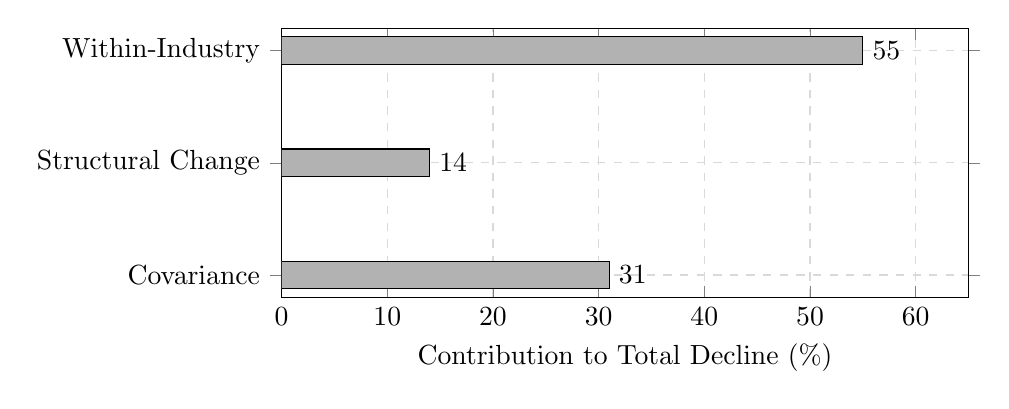
\begin{tikzpicture}
    \begin{axis}[
        xbar,
        width=0.85\textwidth,
        height=5cm,
        symbolic y coords={Covariance, Structural Change, Within-Industry},
        ytick=data,
        xlabel={Contribution to Total Decline (\%)},
        xmin=0, xmax=65,
        nodes near coords,
        nodes near coords align={horizontal},
        grid=major,
        major grid style={dashed, gray!30}
    ]
    \addplot[fill=gray!60, draw=black] coordinates {(55,Within-Industry) (14,Structural Change) (31,Covariance)};
    \end{axis}
\end{tikzpicture}
\caption{Visualizing the Decomposition. The Covariance term (31\%) is unusually high, indicating a synchronized shock.}
\label{fig:decomp}
\end{figure}
% ----------------------------------------------------------

\bigskip

\paragraph{Analytical Implication}
The decomposition reveals that the decline is not monocausal. The 55\% Within-Industry contribution validates the search for a pervasive force affecting production functions (like RPI or markups). However, the combined 45\% contribution of Structural Change and Covariance indicates that the macroeconomic reallocation of resources is equally vital.

The large 31\% Covariance Term is particularly diagnostic. It signifies that the sectors driving India’s growth (specifically Services) were not merely expanding; they were fundamentally altering their production structures to become less labor-intensive. This points towards a unified shock that promotes both capital deepening (lowering $ls_i$) and output expansion (raising $v_i$).

\newpage
% ----------------------------------------------------------
\section{Econometric Estimation of Markups: Methodological Rigor}

Before constructing the theoretical model, it is imperative to empirically test the Rising Markup hypothesis. Since data on Indian markups is sparse, particularly for the pre-2000 period, Sinha (2023) undertakes a primary econometric estimation using firm-level data from the Annual Survey of Industries (ASI).

\subsection{The Challenge of Endogeneity}
Estimating production functions is notoriously difficult due to simultaneity bias (endogeneity). Firms observe their own productivity shocks ($\omega_{it}$) and adjust their variable inputs (like labor and materials) accordingly. However, the econometrician does not observe $\omega_{it}$. Consequently, a simple OLS regression of output on inputs will yield biased coefficients, as the inputs are correlated with the error term.

To address this, Sinha employs the Olley–Pakes (1996) control function approach \citep{OlleyPakes1996}. This methodology assumes that a firm's investment decision is a strictly increasing function of its productivity and capital stock: $i_{it} = f(k_{it}, \omega_{it})$. By inverting this function, productivity can be expressed as a function of observable investment and capital: $\omega_{it} = f^{-1}(i_{it}, k_{it})$. This allows the unobserved productivity shock to be proxied by observables, recovering consistent estimates of the production function parameters.

\subsection{Implementation and Proxy Variables}
Sinha implements the Olley–Pakes estimator using the \texttt{prodest} function in Stata. The estimation specification is:

\[
y_{it} = \beta_l l_{it} + \beta_k k_{it} + \beta_m m_{it} + \omega_{it} + \epsilon_{it}
\]

where $y$ is gross sales, $k$ is total capital, and the intermediate input $m$ (cost of production) is treated as the static variable input. Investment is used as the proxy variable for productivity.

\paragraph{Robustness Checks}
Recognizing the limitations of investment as a proxy (e.g., zero-investment observations are dropped, leading to selection bias), the analysis also explores alternative proxies such as intermediate energy inputs, following Levinsohn and Petrin (2003) \citep{LevinsohnPetrin2003}. The snippet analysis indicates that using labor employment or intermediate inputs yields variations in markup levels, but the central trend remains robust.

\subsection{Empirical Findings: The Markup Trajectory}
The markup $\mu_{it}$ is calculated from the estimated output elasticity of the variable input ($\beta_m$) and the share of that input in revenue ($s_{mit}$):

\[
\mu_{it} = \frac{\beta_m}{s_{mit}}
\]

\paragraph{Key Results}
\begin{enumerate}[leftmargin=*,itemsep=4pt]
\item \textbf{Level:} The average markup for the Indian manufacturing sector in the period 2003–2007 is estimated at 1.22 (22\%).
\item \textbf{Trend:} Crucially, the analysis finds no evidence of a secular upward trend in markups post-2000. While there are cyclical fluctuations—markups rose to 1.33 prior to the Great Recession and fell to 1.16 thereafter—there is no persistent rise comparable to the US experience documented by De Loecker et al. (2020) \citep{DeLoecker2020}.
\item \textbf{Historical Inference:} Regarding the 1980s, Sinha argues based on the industrial organization literature that the pre-reform Indian economy was characterized by high concentration and barriers to entry. Therefore, it is reasonable to assume that markups in 1980 were at least as high as 1.22, if not higher. This challenges the applicability of the Rising Markup hypothesis (which relies on markups increasing from near 1.0) to the Indian context.
\end{enumerate}

\newpage
% ----------------------------------------------------------
\section{The General Equilibrium Framework: Modeling the Indian Economy}

To disentangle the causal drivers and simulate counterfactuals, Sinha (2023) constructs a three-sector General Equilibrium (GE) model. This model is the analytical engine of the research, designed to capture the specific structural features of the Indian economy.

\subsection{Production: The CES Architecture}
The economy consists of three sectors: Agriculture ($A$), Manufacturing ($M$), and Services ($S$). In each sector, production occurs in two stages:
\begin{enumerate}[leftmargin=*,itemsep=4pt]
\item \textbf{Intermediate Goods:} A continuum of monopolistically competitive firms produce differentiated intermediate varieties.
\item \textbf{Final Goods:} Perfectly competitive assemblers bundle these varieties into sectoral final goods.
\end{enumerate}

The core technology is the Constant Elasticity of Substitution (CES) production function used by intermediate firms:

\[
Y_{it} = \left[ \alpha_i K_{it}^{\frac{\sigma_i-1}{\sigma_i}} + (1-\alpha_i) L_{it}^{\frac{\sigma_i-1}{\sigma_i}} \right]^{\frac{\sigma_i}{\sigma_i-1}}
\]

The Role of $\sigma_i$:
\begin{itemize}[leftmargin=*,itemsep=4pt]
\item If $\sigma_i > 1$, capital and labor are gross substitutes. A fall in the cost of capital ($R$) leads to a more-than-proportional increase in capital usage, causing the labor share to fall.
\item If $\sigma_i < 1$, capital and labor are gross complements. A fall in $R$ leads to a less-than-proportional increase in $K$, causing the labor share to rise.
\end{itemize}

Unlike many studies that assume a value for $\sigma$, Sinha calibrates these elasticities to match the observed changes in labor shares in India, ensuring the model is disciplined by the data.

\subsection{Demand: Non-Homothetic Preferences (Stone--Geary)}
A central innovation of the model is the use of non-homothetic preferences to generate endogenous structural transformation. Standard Cobb--Douglas preferences would imply constant expenditure shares across sectors regardless of income, which contradicts the Indian experience of rapid sectoral reallocation.

Sinha employs a Stone--Geary utility function:

\[
U(C_A, C_M, C_S) = (C_A - \bar{a})^{\gamma_A} C_M^{\gamma_M} C_S^{\gamma_S}
\]

\paragraph{The Subsistence Constraint ($\bar{a}$)}
The term $\bar{a}$ represents the subsistence requirement for agricultural goods (food). Households must strictly satisfy this consumption need before allocating income to manufacturing or services.

\begin{itemize}[leftmargin=*,itemsep=4pt]
\item \textbf{Mechanism:} When the economy is poor (low capital stock), $\bar{a}$ consumes a large fraction of total income. As the economy grows (due to capital accumulation triggered by falling RPI), total income rises. The fixed subsistence expenditure $\bar{a}$ becomes a smaller share of the budget, and marginal income is directed toward Manufacturing and Services (governed by $\gamma_M$ and $\gamma_S$).
\item \textbf{Calibration:} The parameter $\bar{a}$ is calibrated to match the high value-added share of Agriculture in 1980 (36\%). The weights $\gamma$ are calibrated to match the shares of other sectors.
\end{itemize}

This preference structure creates a theoretical link between the RPI decline and structural change. The cheapening of investment goods increases real income, which pushes the economy away from the subsistence constraint, naturally expanding the Services sector.

\subsection{Equilibrium Conditions}
The model closes with standard market-clearing conditions:
\begin{itemize}[leftmargin=*,itemsep=4pt]
\item \textbf{Labor Market:} $\sum_i L_{it} = \bar{L}$ (Labor is mobile across sectors, implying a unified wage $W$).
\item \textbf{Capital Market:} $\sum_i K_{it} = K_t$ (Capital is rented at rate $R$).
\item \textbf{Goods Markets:} Output equates to consumption plus investment ($Y_M = C_M + X$).
\item \textbf{Investment:} The investment good $X$ is produced from manufacturing output using a linear technology $A_x$. The price of investment is $q_t = 1/A_{xt}$. A rise in $A_x$ (technical progress) lowers $q_t$ (the RPI).
\end{itemize}

\newpage
% ----------------------------------------------------------
\section{Quantitative Analysis: The Horse Race}

The core of the analysis is a quantitative horse race between two counterfactual scenarios to see which one best replicates the 2007 Indian economy, starting from the 1980 baseline.

\subsection{Scenario 1: The RPI Decline (ISTC Hypothesis)}
\paragraph{The Shock}
The model is subjected only to the observed decline in the Relative Price of Investment (RPI).
\begin{itemize}[leftmargin=*,itemsep=4pt]
\item RPI ($q$): Falls by 47\% (from 1.16 in 1980 to 0.62 in 2007).
\item Markups ($\mu$): Held constant at the estimated level of 1.22 for both periods.
\end{itemize}

\paragraph{Calibration Results}
To match the observed sectoral labor share declines under this shock, the model calibrates the elasticities of substitution as follows:
\begin{itemize}[leftmargin=*,itemsep=4pt]
\item $\sigma_M$ (Manufacturing) = 1.4 (Strong Substitute)
\item $\sigma_S$ (Services) = 1.3 (Substitute)
\item $\sigma_A$ (Agriculture) = 1.05 (Weak Substitute/Cobb--Douglas)
\end{itemize}

\paragraph{Model Performance}
\begin{enumerate}[leftmargin=*,itemsep=4pt]
\item \textbf{Aggregate Fit:} The model predicts a 6.6 percentage point decline in the aggregate labor share. This explains 96\% of the actual 6.8 pp decline observed in the data.
\item \textbf{Structural Change:} The model endogenously generates a massive shift in value-added shares. The share of Agriculture falls from 36\% to 21\% (Data: 18\%), and the share of Services rises from 50\% to 61\% (Data: 66\%). This is driven entirely by the income effect of capital deepening releasing households from the subsistence constraint.
\item \textbf{Covariance:} Crucially, the model generates a covariance term of 16\%, exactly matching the covariance observed in the 3-sector data. The model correctly identifies that the sector growing the fastest (Services) is also substituting capital for labor ($\sigma_S > 1$).
\end{enumerate}
\newpage
\subsection{Scenario 2: RPI Decline + Rising Markups (Market Power Hypothesis)}
\paragraph{The Shock}
The model is subjected to the RPI decline plus a hypothetical increase in markups.
\begin{itemize}[leftmargin=*,itemsep=4pt]
\item RPI ($q$): Falls by 47\%.
\item Markups ($\mu$): Rise from 1.0 (perfect competition) in 1980 to 1.22 in 2007.
\end{itemize}

\paragraph{Calibration Results}
To match the observed 2007 labor shares given the additional downward pressure from rising markups, the calibrated elasticities must change drastically:
\begin{itemize}[leftmargin=*,itemsep=4pt]
\item $\sigma_M = 1.2$ (Substitute)
\item $\sigma_S = 0.85$ (Complement)
\item $\sigma_A = 0.59$ (Complement)
\end{itemize}

\paragraph{The Reversal Effect}
This is a critical theoretical finding. Because the markup increase puts such immense downward pressure on the labor share, the model forces the production function to become complementary ($\sigma < 1$) in Agriculture and Services to prevent the labor share from falling too much.
\begin{itemize}[leftmargin=*,itemsep=4pt]
\item When $\sigma < 1$, a fall in RPI (cheaper capital) actually raises the labor share.
\item Thus, in this scenario, the RPI decline acts as a countervailing force against the markup shock.
\end{itemize}

\paragraph{Model Performance}
\begin{enumerate}[leftmargin=*,itemsep=4pt]
\item \textbf{Aggregate Fit:} The model predicts a decline of 5.8 percentage points, explaining only 84\% of the actual decline.
\item \textbf{Covariance Failure:} The covariance term collapses to 5\%. The rising markup acts as a tax on the economy, suppressing the income growth required to drive the structural transformation. Consequently, the model fails to replicate the rapid expansion of the Service sector.
\item \textbf{Labor Allocation:} The model incorrectly predicts the direction of factor movements, failing to capture the magnitude of labor reallocation from Agriculture to Services.
\end{enumerate}

\subsection{Verdict}
The analysis overwhelmingly favors Scenario 1. The RPI-only model is parsimonious, fits the aggregate data better (96\% vs 84\%), and crucially, captures the internal dynamics of the transition (the covariance term and structural shift). The Rising Markup hypothesis requires implausible assumptions about 1980s market structure (perfect competition) and forces the model into a regime of gross complementarity ($\sigma < 1$) that contradicts the broad consensus on modern production technologies.

% ----------------------------------------------------------
% GRAPH 4: HORSE RACE RESULTS (CORRECTED)
% ----------------------------------------------------------
\begin{figure}[H]
\centering
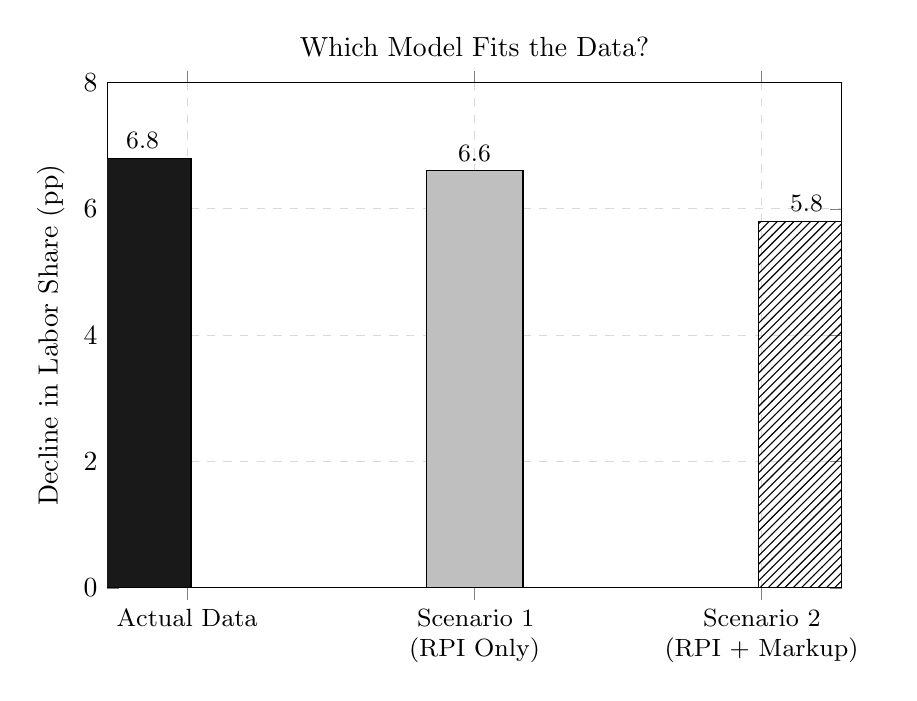
\begin{tikzpicture}
    \begin{axis}[
        ybar,
        bar width=35pt,
        width=0.9\textwidth,
        height=8cm,
        % -----------------------------------------------------------
        % FIX: We use numbers 1, 2, 3 for positions.
        % This prevents "Package PGF Math Error" caused by text mismatches.
        % -----------------------------------------------------------
        xtick={1, 2, 3},
        xticklabels={Actual Data, Scenario 1\\(RPI Only), Scenario 2\\(RPI + Markup)},
        xticklabel style={align=center, text width=3cm, font=\small, anchor=north},
        enlarge x limits=0.3,
        ylabel={Decline in Labor Share (pp)},
        ymin=0, ymax=8,
        % y dir=reverse,  <-- REMOVED to make bars go UP
        grid=major,
        major grid style={dashed, gray!30},
        title={Which Model Fits the Data?},
        nodes near coords,
        nodes near coords style={font=\small}
    ]

    % Plot 1 (Position 1)
    \addplot[
        fill=black!90,
        draw=black,
        nodes near coords style={text=black}
    ] coordinates {(1.2, 6.8)};

    % Plot 2 (Position 2)
    \addplot[
        fill=gray!50,
        draw=black,
        nodes near coords style={text=black}
    ] coordinates {(2, 6.6)};

    % Plot 3 (Position 3)
    \addplot[
        pattern=north east lines,
        pattern color=black,
        draw=black,
        nodes near coords style={text=black}
    ] coordinates {(2.8, 5.8)};

    \end{axis}
\end{tikzpicture}
\caption{The Horse Race: Explained variation of the aggregate decline. Scenario 1 (RPI Only) provides the superior fit.}
\label{fig:horserace}
\end{figure}
% ----------------------------------------------------------

\newpage
% ----------------------------------------------------------
\section{Critical Limitations: The Missing Middle and the Informal Sector}

While Sinha (2023) provides a coherent framework for the formal economy, a comprehensive review must address the limitations imposed by the exclusion of the informal sector.

\subsection{The Dual Economy Dilemma}
The Indian economy is a dual economy structure. The KLEMS and ASI data primarily capture the organized sector. However, the unorganized or informal sector accounts for:
\begin{itemize}[leftmargin=*,itemsep=4pt]
\item \textbf{Employment:} Over 90\% of the total workforce.
\item \textbf{Manufacturing Employment:} Nearly 80\% of manufacturing employment, despite producing only 30\% of output.
\end{itemize}

\paragraph{Implications for Analysis}
\begin{enumerate}[leftmargin=*,itemsep=4pt]
\item \textbf{Capital Intensity:} Informal firms are typically labor-intensive and credit-constrained. They face a higher effective cost of capital than formal firms. The transmission mechanism of the RPI decline (cheaper global machinery) may not reach these firms, meaning the substitution effect ($\sigma$) is likely much lower (or close to zero) in the informal sector.
\item \textbf{Labor Share Stability?} It is plausible that the labor share in the informal sector has remained stable or behaved differently. If the informal sector acts as a sink for surplus labor with stagnant wages and minimal capital, the aggregate decline observed in KLEMS might overstate the capital deepening of the average Indian worker's experience, while accurately reflecting the corporate Indian experience.
\item \textbf{Contract Labor:} A bridging phenomenon is the rise of informal workers in the formal sector (contract labor). Snippets indicate that strict labor laws (Industrial Disputes Act) encourage formal firms to hire contract workers to avoid regulatory rigidity. This creates a flexible labor margin. If formal firms substitute permanent workers (high cost) for contract workers (low cost) or capital, this manifests as a decline in the formal labor share.
\end{enumerate}
\newpage
\subsection{The Aggregation Gap}
The drop in the covariance term from 31\% (27 industries) to 16\% (3 sectors) suggests that Services is too broad a category. Future research needs to disaggregate Services into Modern (IT, Finance) and Traditional components. The RPI hypothesis likely fits the Modern component perfectly, while the Traditional component may be driven by different forces (e.g., Lewisian surplus labor).

\newpage
% ----------------------------------------------------------
\section{Conclusion and Policy Implications}

\subsection{Synthesis of Findings}
This exhaustive analysis of the decline of the labor share in India leads to several robust conclusions:
\begin{enumerate}[leftmargin=*,itemsep=4pt]
\item \textbf{Technological Dominance:} The primary driver of the decline is the Investment-Specific Technical Change (ISTC), manifested as a sharp, policy-induced reduction in the Relative Price of Investment following the 1991 liberalization.
\item \textbf{Substitution and Income Effects:} This price shock unleashed two simultaneous forces: a substitution effect (driving down labor shares within formal industries) and an income effect (driving structural transformation from agriculture to services).
\item \textbf{Rejection of Rising Markups:} There is no empirical evidence of a secular rise in markups in India's formal manufacturing sector post-2000, and the markup hypothesis fails to replicate the structural dynamics of the economy in general equilibrium.
\end{enumerate}

\subsection{Policy Implications}
For policymakers, these findings suggest that the falling labor share is, to a significant extent, a byproduct of modernization and efficiency. The decline reflects the integration of Indian industry with global technology frontiers (adopting capital-intensive methods). Policies attempting to artificially prop up the labor share (e.g., through rigid employment protection) might be counterproductive if they impede the capital accumulation that drives the income growth necessary for structural transformation.

However, the findings also highlight a distributional challenge. If the engine of India's growth (Modern Services and Manufacturing) is structurally shifting income away from labor, reliance on growth alone to reduce inequality is insufficient. The challenge lies in managing the transition: ensuring that the productivity gains from capital deepening are reinvested in human capital, allowing the workforce to access the high-skill roles complementary to the new capital stock, rather than being stranded in the low-productivity informal sector.

\subsection{Future Research}
The frontier of this research lies in closing the data gap on the informal sector. Integrating the unorganized economy into these sophisticated General Equilibrium models is the necessary next step to produce a truly holistic understanding of inequality in India.

\newpage
% ----------------------------------------------------------

\addcontentsline{toc}{section}{References}


\begin{thebibliography}{99}

\bibitem{Ackerberg2015}
Ackerberg, D. A., Caves, K., \& Frazer, G. (2015).
\newblock Identification Properties of Recent Production Function Estimators.
\newblock \emph{Econometrica}, 83(6), 2411--2451.

\bibitem{Chaurey2015}
Chaurey, R. (2015).
\newblock Labor regulations and contract labor use: Evidence from Indian firms.
\newblock \emph{Journal of Development Economics}, 114, 224--232.

\bibitem{Chirinko2008}
Chirinko, R. S. (2008).
\newblock $\sigma$: The long and short of it.
\newblock \emph{Journal of Macroeconomics}, 30(2), 671--686.

\bibitem{DeLoecker2020}
De Loecker, J., Eeckhout, J., \& Unger, G. (2020).
\newblock The Rise of Market Power and the Macroeconomic Implications.
\newblock \emph{The Quarterly Journal of Economics}, 135(2), 561--644.

\bibitem{Goldar2013}
Goldar, B. (2013).
\newblock Organised Manufacturing Employment in India: Trends and Determinants.
\newblock \emph{Economic and Political Weekly}.

\bibitem{HsiehKlenow2014}
Hsieh, C.-T., \& Klenow, P. J. (2014).
\newblock The Life Cycle of Plants in India and Mexico.
\newblock \emph{The Quarterly Journal of Economics}, 129(3), 1035--1084.

\bibitem{JohriRahman2022}
Johri, R., \& Rahman, A. (2022).
\newblock The Rise and Fall of India's Relative Investment Price.
\newblock Working paper / CAFRAL analysis.

\bibitem{Karabarbounis2013}
Karabarbounis, L., \& Neiman, B. (2013).
\newblock The global decline of the labor share.
\newblock \emph{Quarterly Journal of Economics}.

\bibitem{LevinsohnPetrin2003}
Levinsohn, J., \& Petrin, A. (2003).
\newblock Estimating Production Functions Using Inputs to Control for Unobservables.
\newblock \emph{Review of Economic Studies}.

\bibitem{OlleyPakes1996}
Olley, G., \& Pakes, A. (1996).
\newblock The Dynamics of Productivity in the Telecommunications Equipment Industry.
\newblock \emph{Econometrica}.

\end{thebibliography}

\end{document}